\ProvidesPackage{commands}
\documentclass[11pt]{report}
\usepackage{epstopdf}
\usepackage{amsmath}
\usepackage{epsf}
\usepackage{amsfonts}
\usepackage{amssymb}
\usepackage{color}
\usepackage{mathtools}
\usepackage{placeins}
\usepackage{booktabs}
\usepackage{enumitem}
\usepackage{caption}
\usepackage[margin=0.7in, paperwidth=8.5in, paperheight=11in]{geometry}
\usepackage{amsfonts}
\usepackage{amsbsy}
\usepackage{authblk}
\usepackage{listings}
\usepackage{array}
\usepackage{titlesec}
\usepackage{bm}
\usepackage{titlesec}
\usepackage{empheq}
\usepackage[latin1]{inputenc}
\usepackage{mathtools}
\usepackage{graphicx}
\usepackage{caption}
\usepackage{subcaption}
\usepackage{multicol}
\usepackage{xspace}
\usepackage{hyperref}
\usepackage{url}
\usepackage{natbib}


\newcommand{\del}[2]{\frac{\partial {#1}}{\partial {#2}}}
\newcommand{\D}[2]{\frac{D^{\overline{\alpha}}}{\overline{\alpha !}}{#1}(#2,#2)\ {\bf x}^{\overline{\alpha}}}
\newcommand{\dv}[3]{\frac{{\rm d}^{#1}{#2}}{d{#3}^{#1}}}
\newcommand{\ddel}[5]{\frac{\partial^{ {#1} + {#2}} {#3}}{\partial {#4}^{#1} \partial{#5}^{#2}}}
\newcommand{\dev}{{\rm {\bf dev}}}
\newcommand{\proj}[1]{\frac{1}{R^2}{\bf X}\otimes{\bf X}}
\newcommand{\Ie}[1]{I^{\rm e}_{#1}}
\newcommand{\Ce}[1]{\bf C^{\rm e^{#1}}}
\newcommand{\Fe}[2]{F^{\rm e^{#2}}_{#1}}
\newcommand{\Fv}[2]{F^{\rm v^{#2}}_{#1}}
\newcommand{\C}[2]{C^{\rm {#2}}_{#1}}
\newcommand{\f}[2]{f^{\rm {#2}}_{#1}}
\newcommand{\B}[2]{B^{\rm {#2}}_{#1}}
\newcommand{\E}[2]{E^{\rm {#2}}_{#1}}
\newcommand{\fv}[2]{f^{\rm v^{#2}}_{#1}}
\newcommand{\dfv}[2]{\dot{f}^{\rm v^{#2}}_{#1}}
\newcommand{\tGam}[2]{\tilde{\Gamma}^{\rm v^{#2}}_{#1}}
\newcommand{\Gam}[2]{\Gamma^{\rm v^{#2}}_{#1}}
\newcommand{\A}[1]{\mathcal{A}_{#1}}
\newcommand{\F}[2]{F^{\rm #2}_{#1}}
\newcommand{\hpeq}{\hat{\psi}^{\rm Eq}}
\newcommand{\hpneq}{\hat{\psi}^{\rm NEq}}
\newcommand{\etak}{\eta_K({I_1,I_2,J},{\bf C^{\rm e}, B^{\rm v}})}
\newcommand{\nuk}{\nu_K({I_1,I_2,J},{\bf C^{\rm e}, B^{\rm v}})}
\newcommand{\thetak}{\theta_K({I_1,I_2,J},{\bf C^{\rm e}, B^{\rm v}})}
\newcommand{\etaj}{\eta_J({I_1,I_2,J},{\bf C^{\rm e}, B^{\rm v}})}
\newcommand{\dFv}[2]{\dot{F}^{\rm v^{#2}}_{#1}}
\newcommand{\hatpsi}{\widehat{\psi}(I_1, I_2,I^{\rm e}_1,I^{\rm e}_2,J)}
\newcommand{\hpsi}{\widehat{\psi}(I_1,I^{\rm e}_1,J)}
\newcommand{\Fh}[1]{\widehat{\mathcal{F}}\left({\bf F, \Fv{}{}}, {#1}\right)}
\newcommand{\Fhstar}[1]{\widehat{\mathcal{F}}^*\left({\bf F, \Fv{}{}}, {#1}\right)}
\newcommand{\sbar}{\overline{\bm{\sigma}}}
\newcommand{\hpsicomp}[1]{\sum_{r=1}^{2}\left\{\frac{3^{1-\alpha_r}}{2\alpha_r}\mu_r(I^{\alpha_r}_1-3^{\alpha_r})
+\frac{3^{1-a_r}}{2a_r}m_r({\Ie{1}}^{^{a_r}}-3^{a_r})\right\}
+\mu{#1}+\kappa{#1}^2}
\newcommand{\Ni}[1]{N^{(e)}_i(#1)}
\newcommand{\hNi}[1]{\hat{{N}}^{(e)}_i(#1)}
\newcommand{\Ld}{L^{\dagger}}
\newcommand{\intinfinf}{\int_{-\infty}^{\infty} \int_{-\infty}^{\infty}}
\newcommand{\LLnorm}[1]{\left\lVert{#1}\right\rVert_2}
\newcommand{\Linorm}[1]{{\left\lVert{#1}\right\rVert_\infty}}
\newcommand{\tr}{\rm tr}
\newcommand{\deldel}[2]{\frac{\partial^2 {#1}}{\partial {#2}^2}}
\newcommand{\kd}[1]{\delta_{#1}}
\newcommand{\Fie}[1]{{\bf F}^{#1}}
\newcommand{\Comp}{\emph{CompStrainStress\_Cee570.m}}
\newcommand{\Comps}{\emph{CompStrainStress\_Elem\_Cee570.m}}
\newcommand{\Feap}{\emph{FEA\_Program.m}}
\newcommand{\Elast}{\emph{Elast2d\_Elem.m}}
\newcommand{\Assem}{\em{AssemStifForc.m}}
\newcommand{\Fb}{\em{F\_bar\_int}}
\newcommand{\FormFE}{\em{FormFE.m}}
\newcommand{\Sol}{\em{SolveFE.m}}
\newcommand{\inpt}{\em{triangtwo.m}}
\newcommand{\dis}[2]{d^{{#2}}_{#1}}
\newcommand{\vel}[2]{v^{{#2}}_{#1}}
\newcommand\myeq{\stackrel{\mathclap{\normalfont\mbox{def}}}{=}}
\newcommand{\latex}{\LaTeX\xspace}
\newcommand{\tex}{\TeX\xspace}
\newcommand{\vsp}[1]{\\[#1pt]}
\newcommand{\tet}[1]{\texttt{#1}}
\newcommand{\bs}[1]{\boldsymbol{#1}}
\newcommand{\bibtex}{{\sc Bib}\tex}
\newcommand{\biblatex}{{\sc Bib}\latex}
% Matrix Spacing: 
\makeatletter
\renewcommand*\env@matrix[1][\arraystretch]{%
  \edef\arraystretch{#1}%
  \hskip -\arraycolsep
  \let\@ifnextchar\new@ifnextchar
  \array{*\c@MaxMatrixCols c}}
\makeatother

\titlespacing\section{2pt}{12pt plus 4pt minus 2pt}{6pt plus 2pt minus 2pt}
\titlespacing\subsection{2pt}{12pt plus 4pt minus 2pt}{6pt plus 2pt minus 2pt}
\titlespacing\subsubsection{2pt}{12pt plus 4pt minus 2pt}{6pt plus 2pt minus 2pt}
\titlespacing*{\title}{-2ex}{*-2ex}{-2ex}
\usepackage{color} %red, green, blue, yellow, cyan, magenta, black, white
\definecolor{mygreen}{RGB}{28,172,0} % color values Red, Green, Blue
\definecolor{mylilas}{RGB}{170,55,241}
\setlength\parindent{0pt}
\graphicspath{{Figures/}}

\title{Writing a Thesis with \latex}
\author{Bhavesh Shrimali \\ Department of Civil and Environmental Engineering \thanks{Generous Pizza and Coffee Sponsors: ACI and T \& DI}}
\begin{document}
\maketitle
\begin{abstract}
The following work is intended to demonstrate typesetting using \latex. For the purposes of this work, and this work only, it shall be assumed that the reader has no prior knowledge of \latex. However at no point during this work, or the publications that have resulted out of this work, it would be implied that the author(s) is(are) experts in the field. Additionally at all points, whether intentional or unintentional, snide references/remarks to MS-Word shall be made. We hope not to offend any MS-Word fans, but if you get offended we can't help! \vsp{50}
\begin{Huge}
\begin{center}
\latex is AWESOME!!
\end{center}
\end{Huge} 
\end{abstract}
\tableofcontents\newpage
\listoffigures\newpage
\listoftables\newpage
\chapter{\latex Constructs: Basics}
Having stated the important notions relevant to writing a \latex script, we are well positioned to actually start writing a document. The reference for the same is  \cite{lamport1985i1}. Note that although this document is written in a way to mimic a thesis, but it is equally valid in context of writing a research article. It is imperative that we tell \latex kernel the logical and semantic structure of our text. To this end, we consider the most basic work-flow of a \latex script.  
\section{Document Class}
The first thing that you want to tell the kernel is the format of the document you wish to generate. For this document, we specify it to be a "\texttt{report}". The syntax of the command is as follows : \\
\begin{lstlisting}[frame=single]
		\documentclass[Substyle]{sty}
for e.g.	\documentclass[11pt]{report}
\end{lstlisting}
Some important classes (with options) rendered by the \tet{documentclass} command are as follows: 
\begin{itemize}
\item \tet{[11pt]article}, \tet{[11pt, twocolumn]{article}}
\item \tet{book}
\item \tet{report}
\end{itemize}
\section{Preamble}
The space between \texttt{documentclass} and \texttt{begin\{document\}} is called the $Preamble$. It is used to include any packages that might be useful in putting together the document and/or defining any commands to ease our task(s). For a long document, usually, it is beneficial to declare preamble in a separate file, \texttt{commands.tex} in this case, to facilitate easy navigation. A sample of a preamble is as follows: \\
\begin{lstlisting}[frame=single]
		\usepackage{epstopdf}
		\usepackage{amsmath}
		\usepackage{epsf}
		\usepackage{amsfonts}
		\usepackage{amssymb}
		\usepackage{color}
		\usepackage{xspace}
		\usepackage{hyperref}
		\newcommand{\latex}{\LaTeX\xspace}
		\newcommand{\tex}{\TeX\xspace}
\end{lstlisting}\newpage
\section{Title and Author}
It is sometimes beneficial to declare the \texttt{title} and \texttt{author} or the document before actually proceeding to write the body. A sample layout is as follows: \\
\begin{lstlisting}[frame=single]
		\title{Writing a Thesis in \latex}
		\author{Bhavesh Shrimali}
\end{lstlisting}
\section{Document: Main Body}
Once you have declared everything in the preamble, and assigned the \texttt{title} and \texttt{author} we proceed with writing the main body of the document. A sample of the main body is: \\
\begin{lstlisting}[frame=single]
		\begin{document}
			{Main Body}
		\end{document}
\end{lstlisting}
\subsection{Section}
\paragraph{Sections and Subsections}: 
The main body of the document is usually divided in to \tet{section}, \tet{subsection}, \tet{subsubsection} etc. Each of these may further contain text, equations, paragraphs, figures, tables, code-snippets etc. We will now try to go over these in the listed order. A sample of how a section would look like is as follows: 
\begin{lstlisting}[frame=single]
		\section{DocumentClass}
		The first thing that you want to tell the kernel
		is the format of the document you wish to generate.
		For this document, we specify it to be a
		"\texttt{report}". The syntax of the command is as
		follows : \\
\end{lstlisting}
A few important pointers while writing the main body: 
\begin{itemize}
\item Keep a count of the \tet{brackets "\{", "\ [", "\ (" }. Each corresponding bracket should be closed with its dual. 
\item You can include include new lines in the script, however it does not introduce new lines in your document. In order to introduce a newline you have to use a \texttt{DoubleBackSlash}.
\item However when in Math mode, such as \texttt{align} or \texttt{equation}, avoid including new lines as these may result in compilation issues. 
\end{itemize}
\newpage
\subsection{Subsection}
A sample of how a subsection looks like, is as follows. Note that the syntax is exactly the same as a section. : \\
\begin{lstlisting}[frame=single]
		\subsection{Section}
		The main body of the document is usually divided
		in to \tet{section}, \tet{subsection}, 
		\tet{subsubsection} etc. Each of these may further
		contain text, equations, paragraphs, figures, tables,
		code-snippets etc. We will now try to go over these in
		the listed order. A sample of how a section would look
		like is as follows: \\
		\begin{lstlisting}[frame=single]
		\section{DocumentClass}
		The first thing that you want to tell the kernel
		is the format of the document you wish to generate.
		For this document, we specify it to be a
		"\texttt{report}". The syntax of the command is as
		follows : \\
		\end {lstlisting}
\end{lstlisting}
\subsection{Paragraphs}
In line with the previous constructs, paragraphs work in a similar way. A sample layout is as shown below: \\
\begin{lstlisting}[frame=single]
	\subsection{Section}
	\paragraph{Sections and Subsections}: 
	The main body of the document is usually divided 
	into \tet{section}, \tet{subsection}, 	\tet{subsubsection}
	etc. Each of these may further contain text, equations, paragraphs,
	figures, tables, code-snippets etc. 
	We will now try to go over these in the listed order. 
	A sample of how a section would look like is as follows: 
\end{lstlisting}
Some general remarks about Paragraphs in particular, and sections/subsections in general: 
\begin{itemize}
\item Paragraphs, and/or the starting of a new section are generally indented. 
\item In order to remove the indent you should use the \tet{setindent} command; note the other uses also: 
\begin{lstlisting}[frame=single]
		\setlength{\parindent}{0}
		\setlength{\parskip}{2cm plus4mm minus3mm}
or		\noindent {...Paragraph...}
\end{lstlisting}
\item If you want to indent an unindented paragraph use \tet{indent} command: 
\begin{lstlisting}[frame=single]
		\indent{}
\end{lstlisting}
For customized paragraphs we use \tet{verbatim} command. 
\begin{lstlisting}[frame=single]
		\begin{verbatim}
			{Your text.... as it is .. \\ }
		\end{verbatim}
\end{lstlisting}
\end{itemize}
\subsection{URL and HYPERREF}
For typesetting of urls/hyperlinks it is recommended that you use either of the \tet{url} and/or \tet{hyperref} packages. The syntax of both is as follows: \\
\begin{lstlisting}[frame=single]
		\url{<link>}{...text...}
		\hyperref{<link>}{...text...}
\end{lstlisting}
\subsection{Lists}
\latex also allows for the typesetting of lists using a number of inbuilt structures, each of which is marked briefly below. In most cases, for thesis or articles, only \tet{enumerate} and \tet{itemize} are used: \\
\begin{lstlisting}[frame=single]
		\begin{itemize}
		\item Item 1
		\item Item 2
		\end{itemize}
		
		
		\begin{enumerate}
		\item Item 1
		\item Item 2
		\end{enumerate}
\end{lstlisting}
\paragraph{Note:} Additional packages such as \tet{\{ enumerate * \} } are useful in having inline lists in your document. The syntax for these is exactly same as described above for \tet{itemize}.
\chapter{Graphics}
The following chapter is intended to provide a brief overview of the graphics' packages in \latex and their usage in appropriate environments. 
\section{Floats}
Floats are basically things that cannot be broken over a page. Some common examples of floats can be, \tet{table}, \tet{figure} etc. 
\subsection{Figure}
The syntax for \tet{figure} is given below. The \tet{subfigure} package, with the \tet{subfigure}, works similarly: 
\begin{lstlisting}[frame=single]
		\begin{figure}[placement specifier]
			<figure details>
		\end{figure}
\end{lstlisting}
For specifiers we, most commonly use: 
\begin{itemize}
\item \tet{h} - "here", places figure almost at the same point (Not SPOT!)
\item \tet{t} - "top", places figure at the top of the current page
\item \tet{b} - "bottom", places the figure at the bottom of the current page. 
\item \tet{p} - "page", float-only page 
\item \tet{!} - "good", determines the best possible location for the float. 
\end{itemize}
\begin{figure}[!]
\centering
\begin{subfigure}{.5\textwidth}
  \centering
  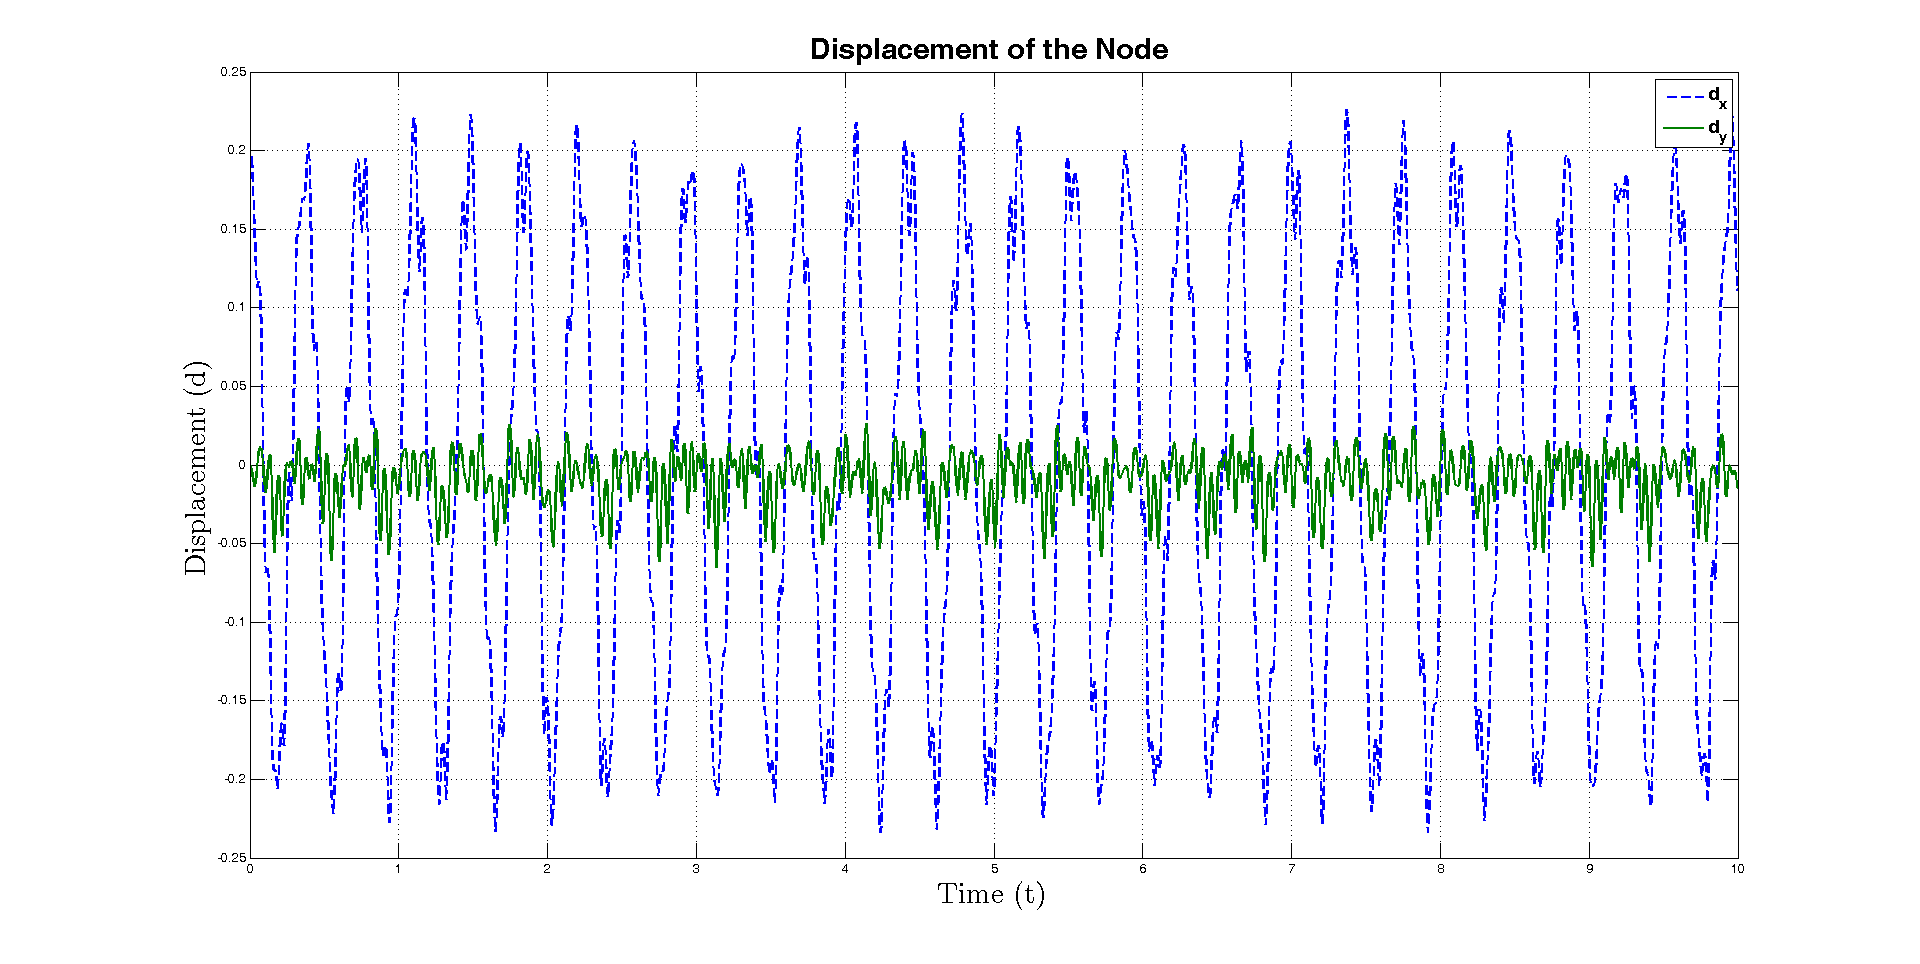
\includegraphics[width=3.5in,height = 4in]{dis4ci}
  \caption{$\Delta t$ = 0.005 , $\alpha = 0$}
  \label{fig:sub1}
\end{subfigure}%
\begin{subfigure}{.5\textwidth}
  \centering
  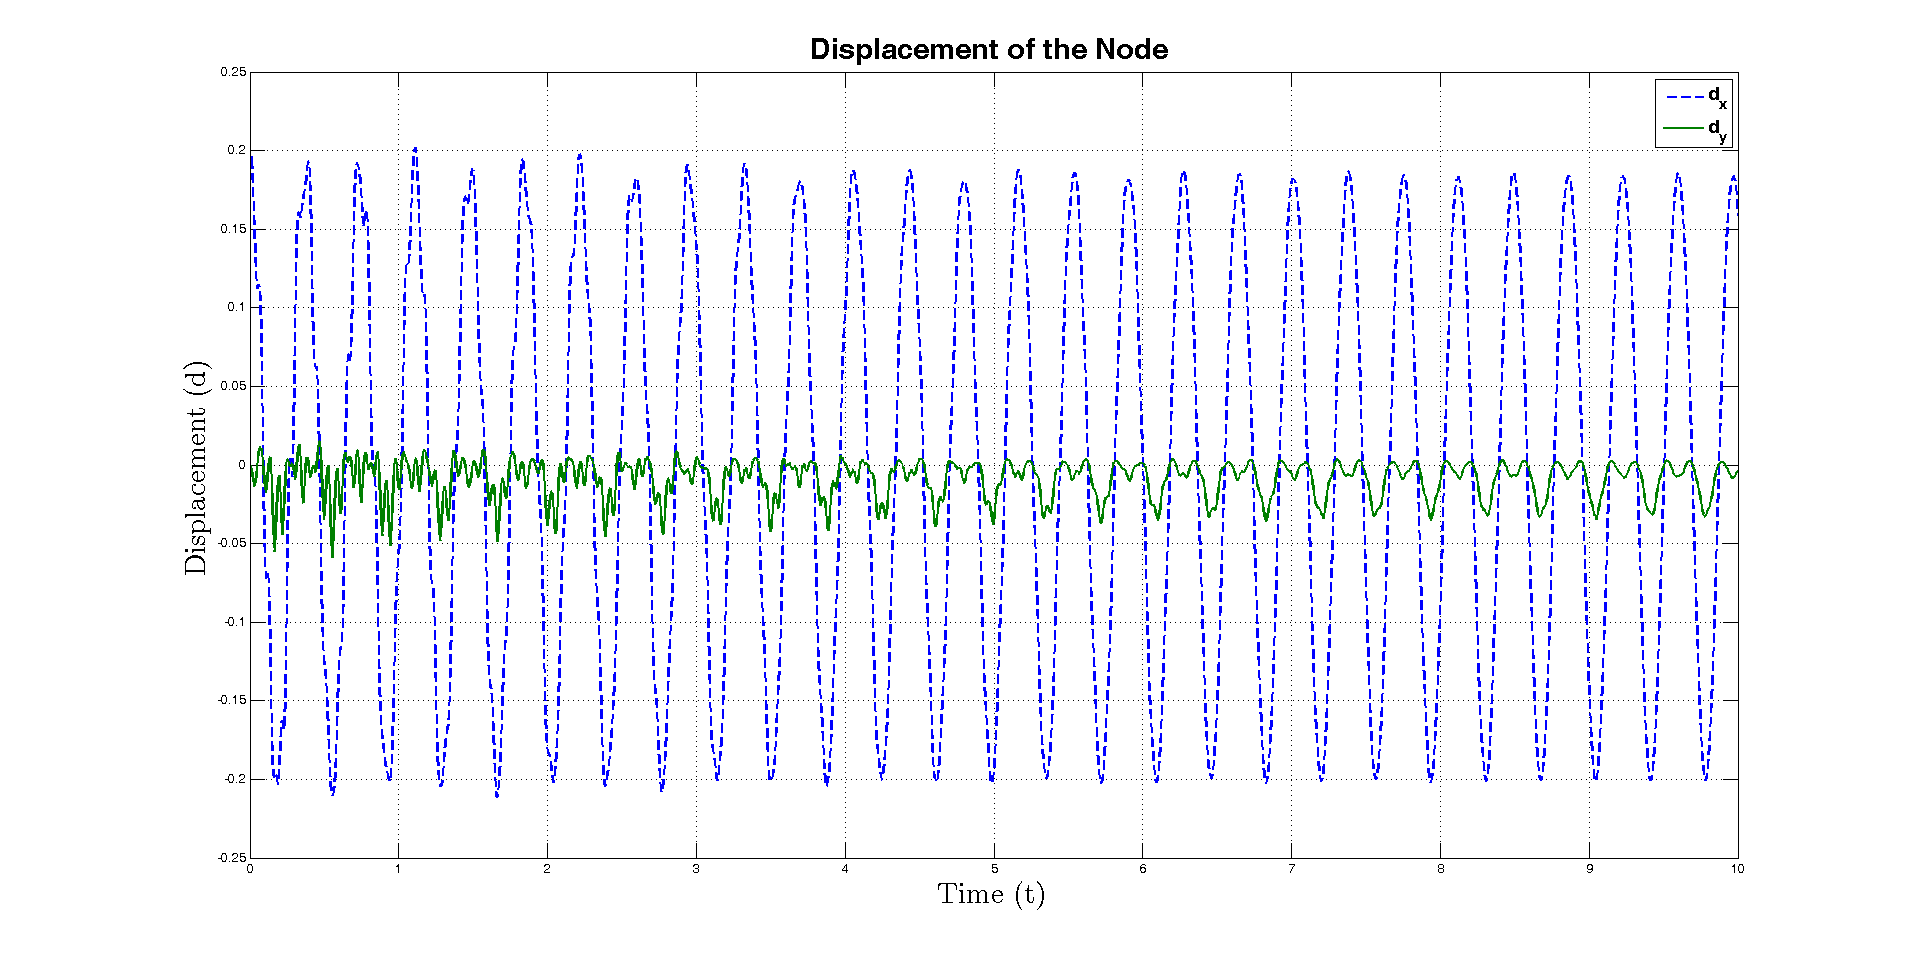
\includegraphics[width=3.5in,height = 4in]{dis4cii}
  \caption{$\Delta t$ = 0.005, $\alpha = -1/3$}
  \label{fig:sub2}
\end{subfigure}
\caption{ Displacement-Time Plots for Shear Loading at Node (3) }
\label{Disp-Shear}
\end{figure}
A sample syntax is as follows: 
\begin{lstlisting}[frame=single]
		\begin{figure}[htbp]
		\centering
		\begin{subfigure}{.5\textwidth}
  			\centering
  			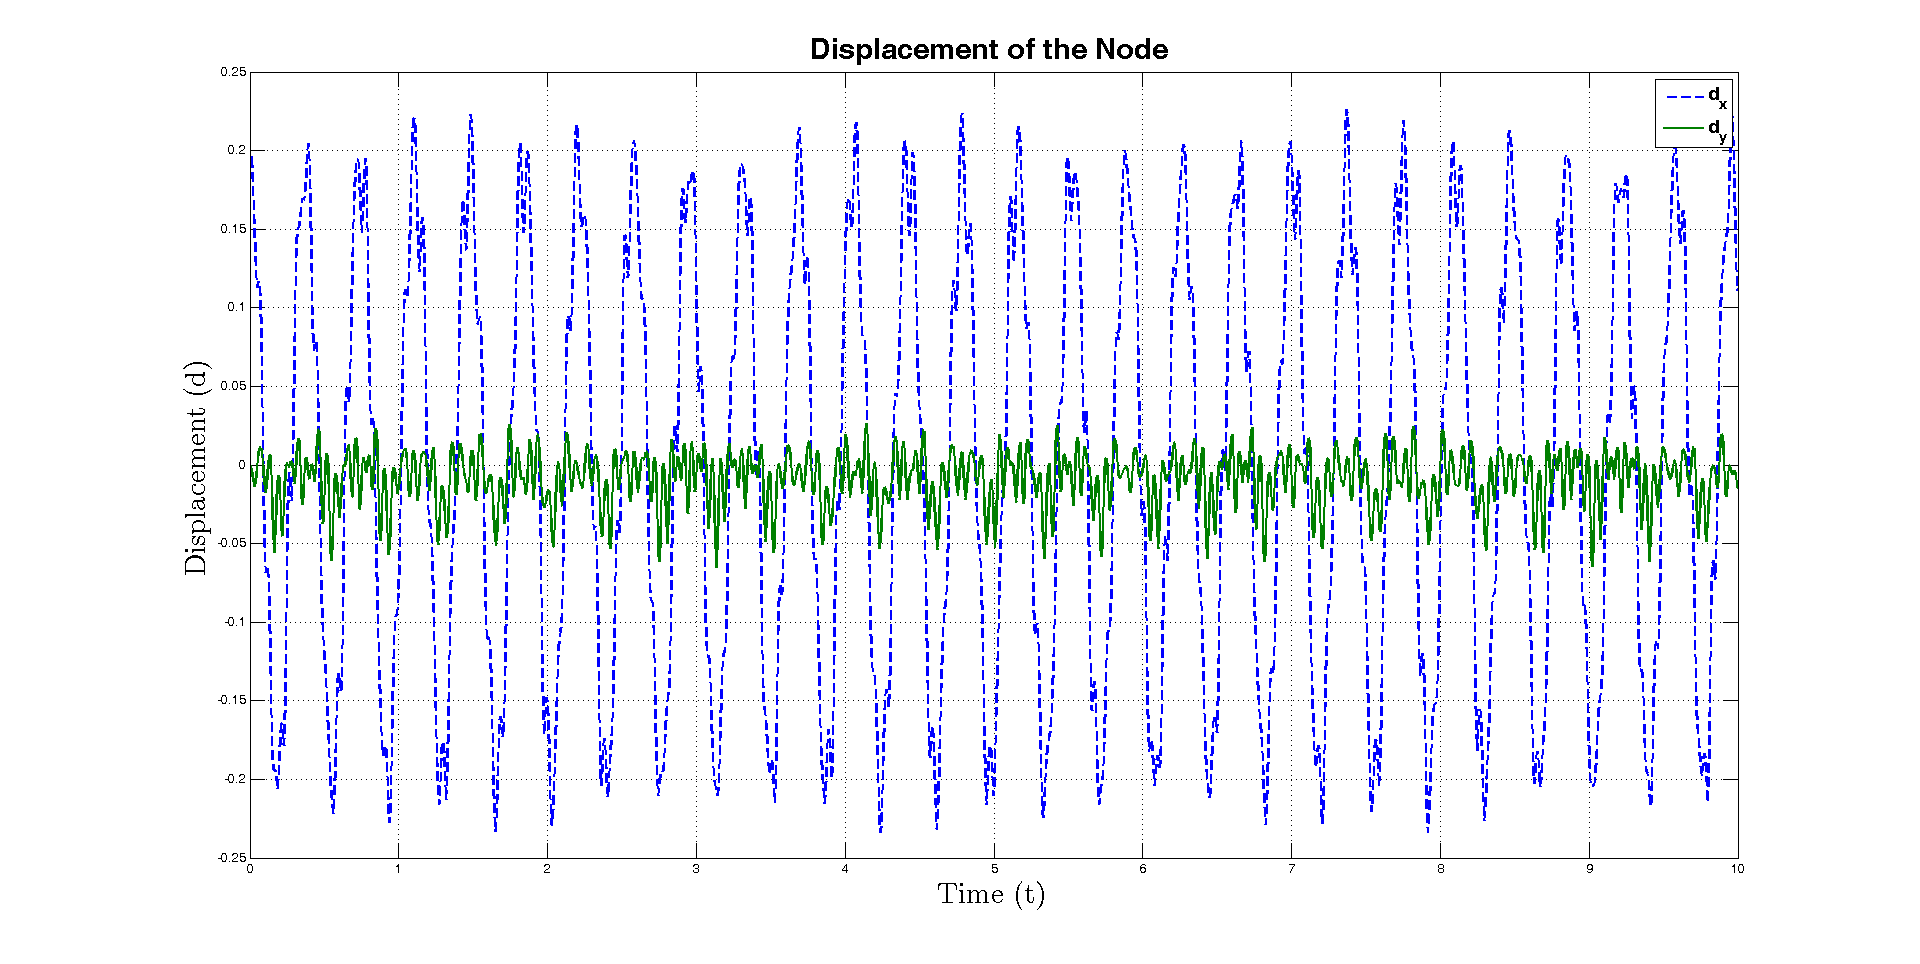
\includegraphics[width=3.5in,height = 4in]{dis4ci}
  		\label{fig:sub1}
		\end{subfigure}%
		\begin{subfigure}{.5\textwidth}
  		\centering
  		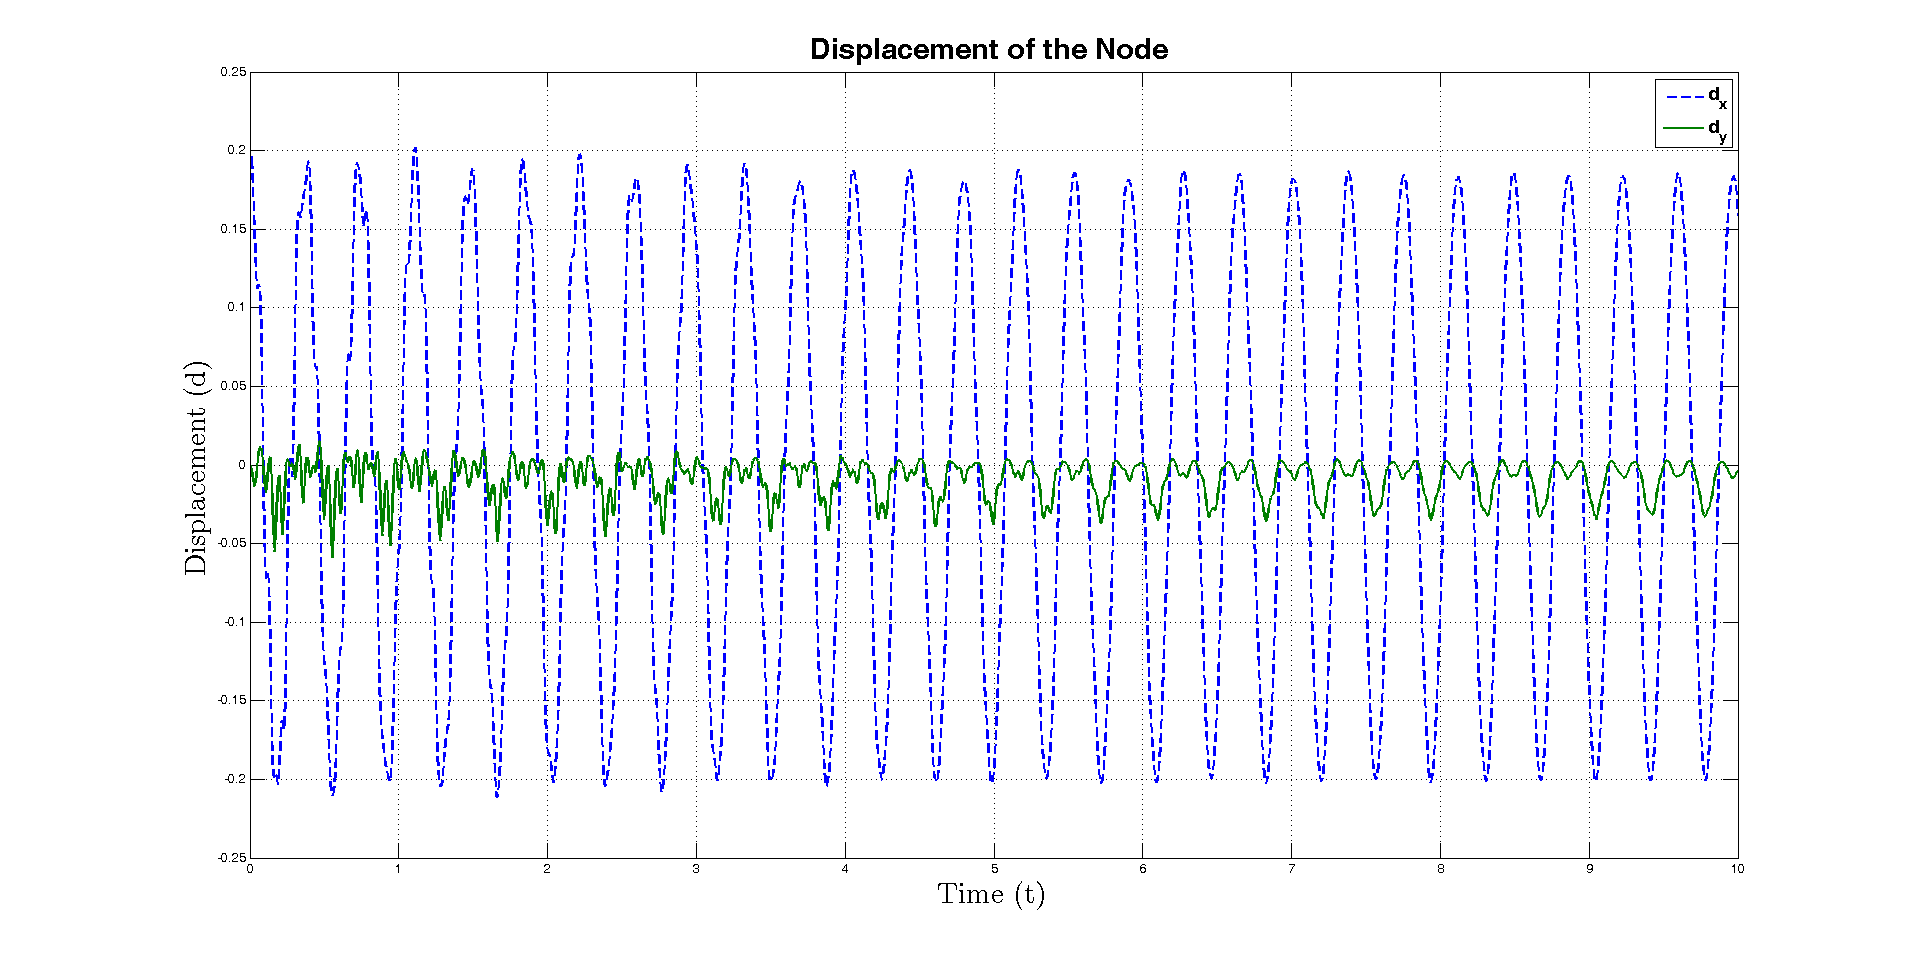
\includegraphics[width=3.5in,height = 4in]{dis4cii}
  		\caption{$\Delta t$ = 0.005, $\alpha = -1/3$}
  		\label{fig:sub2}
		\end{subfigure}
		\label{Disp-Shear}
		\end{figure}
\end{lstlisting}
The following packages are also pre-installed in the preamble to facilitate the rendering of the above figure. 
\begin{itemize}
\item \tet{graphicx} and setting the \tet{graphicspath \{\{\}\}}
\item \tet{caption}
\end{itemize}
Other variants for figures are also possible, for e.g., 
\begin{itemize}
\item \tet{sidecap} package with the command \tet{SCfigure}
\item \tet{subcaption}
\end{itemize}\newpage
\subsection{Table}
\latex can handle tables efficiently but the syntax can  be cumbersome, particularly when large tables are being input. Note, that for a scientific report this may not be the case (sign of bad report if present!) but in general there are several ways to workaround, one of them being \tet{excel2latex} (not efficient without Macros!)
% Table generated by Excel2LaTeX from sheet 'Sheet2'
\begin{table}[ht]
  \centering
  \caption{Custom Caption}
    \begin{tabular}{ccr}
    \toprule
    \textbf{Iter} & \textbf{N = 10} & \multicolumn{1}{c}{\textbf{N = 50}} \\
    \midrule
    \textbf{1} & 3.614743 & 3.839848 \\
    \textbf{2} & 0.089508 & 0.422621 \\
    \textbf{3} & 0.001458 & 0.036089 \\
    \textbf{4} & 3.99E-05 & 0.00397 \\
    \textbf{5} & 6.8E-07 & 0.000346 \\
    \textbf{6} & 1.79E-08 & 3.74E-05 \\
    \textbf{7} & 3.17E-10 & 3.32E-06 \\
    \textbf{8} & 0     & 3.53E-07 \\
    \textbf{9} &       & 3.19E-08 \\
    \textbf{10} &       & 3.34E-09 \\
    \textbf{11} &       & 3.05E-10 \\
    \textbf{12} &       & 0 \\
    \bottomrule
    \end{tabular}%
  \label{table1}
\end{table}
Although the floats in \latex don't seem to be well placed in terms of the default location, it is often easy to manipulate them using macros. (i.e. you can design your own \tet{customtable} environment)
\subsection{Referencing}
The command \tet{listoffigures} takes care of putting together references to whenever the \tet{figure} command is called in the document, referencing the page number and the name of the figure, at the beginning of the report. Similarly the \tet{listoftables} command takes care of putting together all the references to the \tet{table} command in the document, and automatically places them in the start of the document.
\subsection{Additional Notes}
{Special Cases}:
There are additional environments to take into account special cases for floats. (for e.g. \tet{wrapfig}).
\chapter{Math}
The most important and perhaps the most versatile component of \latex is typersetting math. A number of packages such as \tet{amsmath}, \tet{amssymb}, \tet{mathtools} enrich the math environment with a number of additional choices. (such as those required for special characters, in latin, greek alphabets etc. )
\section{Inline Math}
The inline math environment allows for typing in math in-place, i.e. withing your paragraph along with regular text. The syntax for this is as follows: 
\begin{lstlisting}[frame=single]
		regular text ........ $type your math here $ .... regular text
\end{lstlisting}
\section{Out of line Math}
For a number of situations it is required to type in math, in the form of equations, relations etc. for which the inline math environment is unsuitable. There are a number of ways to do this: 
\subsection{Using the Square Brackets}
The syntax for this is as follows: 
\begin{lstlisting}[frame=single]
		\[    \alpha^2 + \beta^2 = \frac{\gamma^2}{4}   \]
\end{lstlisting}
\subsection{Using the Equation environment}
\begin{lstlisting}[frame=single]
		\begin{equation}
			type your equation here ... 
		\end{equation}
\end{lstlisting}
\subsection{Using the align environment}
\begin{lstlisting}[frame=single]
		\begin{align}
			type your equation here ...
		\end{align}
\end{lstlisting}
Note that the \tet{align} and \tet{equation} environments automatically start numbering the equation, for every newline character that they encounter. For equations which need to be skipped for numbering, a \tet{\nonumber} has to be prefixed before the starting of the equation. If there is a good number of equations whose numbering has to be skipped, prefer using \tet{align *} instead. For numbering a group of equations together as one, use the following 
\begin{lstlisting}[frame=single]
		\begin{align}
			\begin{split} 
			
			\end{split}
		\label{ }
		\end{align}
\end{lstlisting}
Note the usage of \tet{label} command. This assigns the set of equations within \tet{split} a single equation label. The next time you want to reference the equation, just use \tet{ref} command with the \tet{label}. Labeling and referencing in \latex follows a common convention across all the environments. 
\section{Symbols}
The most common list of symbols is available \url{https://en.wikibooks.org/wiki/LaTeX/Mathematics}. These need not be memorized as they are available for reference in a number of standard \tet{CTAN} documentation. Most common examples of the ones used are \tet{int} and \tet{sum} commands. 
\section{Matrix Environments}
A number of occasions in reports demand the user to input (show) matrices and vectors. \latex allows for a customized input of these using the \tet{bmatrix}, \tet{Bmatrix} and \tet{vmatrix} environments. The syntax for these is as follows: 
\begin{lstlisting}[frame=single]
	\begin{bmatrix}
		a & b \\
		c & d
	\end{bmatrix}
\end{lstlisting}
Note that the ampersand character (\&) stands for the alignment. It is used in the align environment, in particular, to align the equations with respect to a particular character.(separate for each line)
\chapter{Referencing and BiBTeX}
In all reports, research articles and theses, the list of references is a must have. \latex allows for incorporating this in a multiple ways. \bibtex (or lately BibLaTeX) is a robust tool to incorporate this.
\section{Background}
\bibtex is an auxiliary tool that works to separate bibliography information, from its corresponding presentation, in a thorough and consistent manner. A \bibtex database is stored as a *.bib file (created using any text editor) and is referenced in the main \tex document. \bibtex has been succeeded by \biblatex which follows the same syntax. For this workshop we shall mainly be focusing on \bibtex, and its usage with \latex. The standard syntax followed for a *.bib file is as follows: 
\begin{lstlisting}[frame=single]
		
		@article{thesis,
   		author    = "Shrimali, Bhavesh",
    		title     = "Writing a thesis with LaTeX",
    		journal   = "ACI Workshop",
    		year      = "2017",
		}
\end{lstlisting}
\bibtex knows almost all of the document types that occur in literature, i.e. reports, books, articles. Hence it allows you to completely forget about the formatting as well as the numbering of the references. The syntax for citing a particular document is : 
\begin{lstlisting}[frame=single]
		\cite{}
\end{lstlisting}
There are additional packages such as \tet{natbib} which allow for more flexibility in styling  references. \tet{natbib} allows for a quick and smooth transition between the \emph{Harvard}(author-year) and \emph{numeric} styles. For further reference it is suggested that you look at the references. :)
\paragraph{Note} If you are using \bibtex, the order of compiling your files is very important. For instance. Generally the order is as follows: 
\begin{itemize}
\item \tet{latex} or \tet{pdflatex}
\item \tet{bibtex} \tet{.aux} file(s)
\item \tet{latex} or \tet{pdflatex}
\item \tet{latex} or \tet{pdflatex}
\end{itemize} 
Depending on the number of cross-references \latex should be able to list all the cross-references with two successive compilations. 
\bibliographystyle{plain}
\bibliography{bibsample}
\end{document}